\section{¿El ambiente generaliza a municipios nuevos?}\label{sec:generalizacion}

Para imitar la pregunta de FIRA dejamos fuera del ajuste un municipio completo, lo predijimos solo con variables de
ambiente y repetimos con los nueve municipios. Es una validación por grupos, que mide cómo se comporta un modelo
lejos de sus datos de entrenamiento~\cite{roberts2017}. Usamos ridge y un bosque aleatorio poco profundo, y
reportamos el mejor de los dos (Fig.~\ref{fig:lomo}).

\begin{figure}[t]
\centering
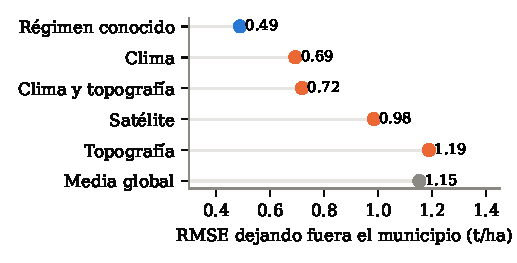
\includegraphics[width=\columnwidth]{r1_generalizacion}
\caption{Error al predecir un municipio que no se vio en el ajuste. El régimen conocido es la referencia: supone que
se sabe el régimen del municipio nuevo.}
\label{fig:lomo}
\end{figure}

El clima predice mejor que la media global (0.69 contra 1.15\,t/ha), pero muy lejos de conocer el régimen (0.49).
Además, esa capacidad no aparece dentro de los regímenes. Con el mismo esquema, aplicado a las parcelas de un solo
régimen, clima y topografía no mejoran la media: 0.536 contra 0.533\,t/ha en el A, y 0.471 contra 0.402 en el B.
Esto significa que el clima predice el nivel del municipio porque distingue la zona norte de la sur, no porque
explique el rendimiento. Con este resultado la pregunta cambia: ¿hay alguna variable del lugar detrás de la brecha?
